% Rules for the HuroCup Penalty Kick Competition
% Jacky Baltes <jacky@cs.umanitoba.ca> 

\documentclass[12pt]{hurocup}

\newcommand{\thisyear}{2010}

\newcommand{\HuroCup}{\textsc{HuroCup}}


\begin{document}

\title{\HuroCup: Penalty Kick\\
  Laws of the Game \thisyear}


\author{Jacky Baltes\\
Autonomous Agents Laboratory\\
University of Manitoba\\
Winnipeg, Manitoba\\
Canada, R3T 2N2\\
Email: jacky@cs.umanitoba.ca\\
WWW: http://www.cs.umanitoba.ca/\~{ }jacky\\[5mm]
Kuo-Yang Tu\\
National Kaohsiung First University of Science and Technology\\
Kaohsiung City, R. O. C.\\
Email: tuky@ccms.nkfust.edu.tw\\
}

\maketitle

\begin{center}
 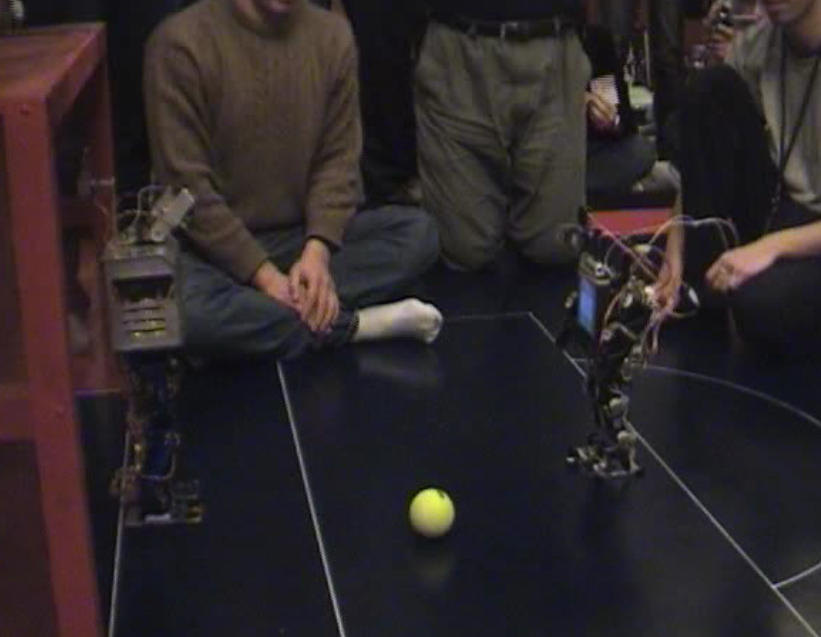
\includegraphics[width=0.7\linewidth]{Figures/penalty-kick-life}
\end{center}

\begin{abstract}
The following rules and regulations govern the penalty kick event in
\HuroCup, a robotic game and robotics benchmark problem for humanoid
robots.
\end{abstract}

\section*{Latest Version of the Rules for \HuroCup\ Penalty Kick}
\label{sec:updates}

The latest official version of the rules of the game for \HuroCup\ is
always available from the \HuroCup\ Facebook page
(http://www.facebook.com/groups/hurocup/).

\section*{Changes to the Rules of \HuroCup\ Penalty Kick for \thisyear}

Some of the penalty kick events will be replaced by Soccer United
competitions in \thisyear.

There are no changes to the \HuroCup\ Penalty Kick rules for \thisyear.

\newpage

\section{Penalty Kick}
\label{sec:penalty-kick}

In this challenge, the robot must approach, dribble a ball into the
shooting zone, and kick a ball into the goal.

\section{Laws of the Game: Penalty Kick}
\label{sec:laws-penalty-kicks}

The following laws describe the specifics of the penalty kick event. For
general specifications relevant to all \HuroCup\ events (e.g., robot
dimensions, playing field and lighting, responsibility of the
referees) please refer to the general \HuroCup\ laws.

\law[PK]{The Field of Play}
\label{pk-field}

\begin{lawlist}[PK]

\item The dimensions of the playing field are at least 220cm by
  180 cm. 

\item One side of the playing field contains a goal. This side of the
  playing field shall be called the goal side. The opposite side of
  the playing field is called the empty side. The two other sides are
  called side lines.

  \begin{figure}
    \begin{center}
      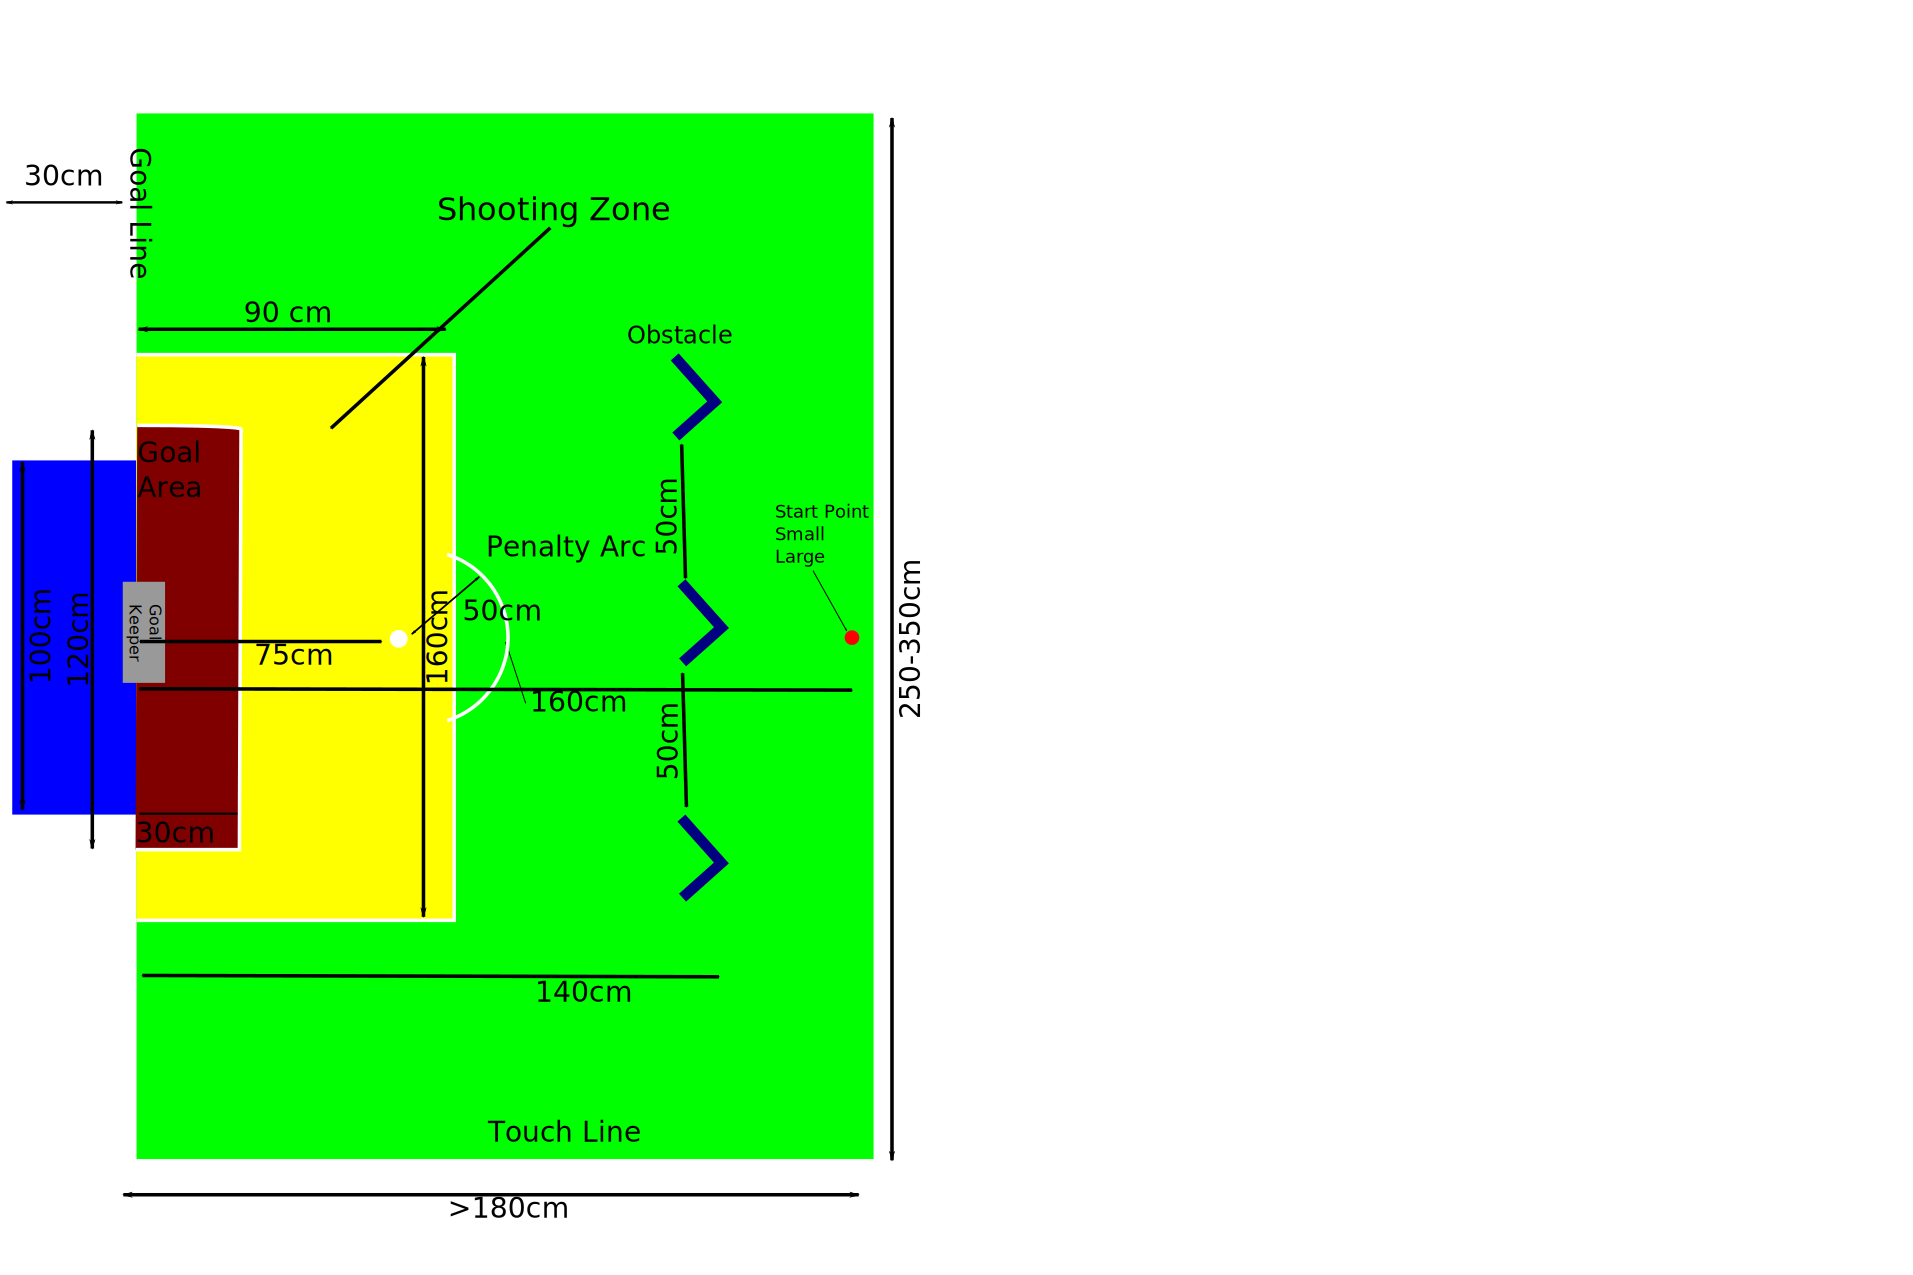
\includegraphics[width=0.7\textwidth]{Figures/penalty-kick}
    \end{center}
    \caption{The field of play for penalty kicks}
    \label{fig:field-penalty}
  \end{figure}

\item The goal is 100cm wide and is placed on the goal side of the
  playing area with its center along the center line of the playing
  field.

\item The penalty mark is 75cm away from the goal line.

\item The penalty area is specified by the triangle that extends from
the penalty mark to the top left and top right corner points of the
goal area.

\item A 120cm wide goal area centered on the goal line extends 30cm
  long into the playing field.

\item A 160cm wide shooting zone centered on the goal line extends
  90cm into the field.
\end{lawlist}

\law[PK]{The Ball}

Please refer to the general \HuroCup\ soccer laws for a description of
the ball.

\law[PK]{Number of Robots}

\begin{lawlist}[PK]
\item A single robot competes in a match.
\end{lawlist}

\law[PK]{The Players}

Please refer to the general \HuroCup\ laws for a description of
the players.

\law[PK]{The Referee}

Please refer to the general \HuroCup\ laws for a description of
the referee.

\law[PK]{The Assistant Referee}

Please refer to the general \HuroCup\ laws for a description of
the assitant referee.
 
\law[PK]{Game Play}

\begin{lawlist}[PK]

\item One robot is designated the kicker, a static goal keeper is
  placed in the goal. All other robots must be positioned behind the
  centre line and must not interfere with the designated kicker or
  goal keeper in any way.

\item The only robots allowed to move during a penalty kick are the
  designated kicker and goal keeper.

\item Each robot may have at most one human handler associated with
  it. 

\item \label{rd-handler1} The human handlers must not interfere in any
  way with other robots, the referee, or other human handlers.

\item \label{rd-handler2} A human handler may only enter the playing
  field or touch his/her robot with the permission of the referee.
  The kick will be declared invalid if the handler touches the robot.

\item The referee will place the ball 160cm away from the goal line
  centered along the goal line and the kicker is placed behind the
  ball.

\item The kicker robot must be at the start point at the beginning of
  the competition. The start point for small and large robots is directly 
behind the ball facing the goal.

\item The designated goal keeper must be positioned so that a part of
 the robot touches the goal line at the start of the game.

\item Three wall obstacles as described in the ``\HuroCup: Obstacle
  Run Laws of the Game \thisyear'' rules will be placed 140cm away
  from the goal line. One obstacle is centered along the goal line and
  the other two obstacles are placed so that the distance between
  obstacles is at least 50cm.

\item The kicker has to move the ball from the start point into the
  shooting zone without touching any of the obstacles. Once the ball
  is completely inside the shooting zone, the kicker must kick the
  ball into the goal.

\item The designated kicker is not allowed to leave the playing field
  or enter the goal area.

\item The designated kicker is not allowed to touch any obstacle.

\item The designated goal keeper is not allowed to leave the goal
area.

\item The designated goal keeper must remain in a standard walking
posture until the ball has been kicked at the goal.

\item Any infringements of the rules shall be dealt with according to
the general \HuroCup\ rules.

\item The penalty kick begins by the referee blowing a whistle.

\item The end of the penalty kick is signaled by the referee by
  blowing the whistle a second time.
  The referee terminates the penalty kick if
  \begin{itemize}
  \item a goal has been scored by the kicker,
  \item the ball is kicked into the goal from outside of the shooting zone,
  \item the ball moved outside of the playing field,
  \item a robot is immobilized by a technical defect,
  \item a robot leaves the playing field,
  \item a robot touches an obstacle,
  \item the maximum duration of the competition (2 minutes) has elapsed,
  \item at least 1 minute has elapsed since the start of the
    competition and it is unlikely in the opinion of the referee that
    the kicker will score in the next minute.
  \end{itemize}

\item After the end of the penalty kick, the next robot is
  designated the kicker.

\end{lawlist}

\law[PK]{Method of Scoring}
\label{penalty-scoring}

\begin{lawlist}[PK]

\item The number of rounds in the competition will be announced at the
  beginning of the competition.

\item Any robot that has not scored a single goal is automatically
  awarded 0 rank.

\item Among the robots that have scored at least one goal, the robots
  are ranked (i.e., 1st place, 2nd place) based on the greater number
  of goals that the robot scored.

\item In case of a tie, i.e., more than one robot having scored the
  same number of goals, the robots will be ranked based on the total
  time required to complete the number of rounds. For example, given
  three robots that scored three goals each with the following times:

      \begin{center}
        \begin{tabular}{l|rrrrr|r|r|}
          \hline
          Robot & \multicolumn{5}{c}{Times} & Total Time & Rank \\
          \hline
          R1 & 30 & 0 & 120 & 110 & 10 & 270 & 3 \\
          R2 & 50 & 50 & 50 & 50 & 50 & 250 & 2 \\
          R3 & 100 & 0 & 0 & 100 & 20 & 220 & 1 \\
          \hline
        \end{tabular}
      \end{center}

  In this example, R3 will be ranked higher than R2, who will be
  ranked higher than R1.

\item The point allocation for robots is as follows:
  \begin{itemize}
  \item The first ranked robot is awarded $10$ points.
  \item The second ranked robot is awarded $8$ points.
  \item The third ranked robot is awarded $6$ points.
  \item The fourth, fifth, sixth, and seventh place robots are awarded
    $4$,$3$,$2$, and $1$ point respectively.  A summary of the point
    allocation for placings is shown in table~\ref{point-allocation}.

    \begin{table}
      \begin{center}
        \begin{tabular}{l|l}
          \hline
          Place & Points scored \\
          \hline
          1 (Winner) & 10 \\
          2          & 8 \\
          3          & 6 \\
          4          & 4 \\
          5          & 3 \\
          6          & 2 \\
          7          & 1 \\
          8, 9, ...  & 0 \\
          \hline
        \end{tabular}
      \end{center}
      \caption{Point allocation for placings in the \HuroCup\ events.}
      \label{point-allocation}
    \end{table}
 \end{itemize}

\item In case of a tie between $n$ robots with rank $k$, all robots
 will be awarded rank $k$ and receive the average of the scores for
 ranks $k$ to $k+n$.  For example, if the robots $A,B,C,D$ scored $10,
 8, 8, 4$ goals respectively, then robot $A$ will be declared the
 winner (1st place) and receive 10 points, both robots $B$ and $C$
 will be declared 2nd place finishers and receive $(8+6)/2=7$, and
 robot $D$ will be declared the fourth place finisher and receive $4$
 points.

\end{lawlist}

\begin{decisions}
\item The goal keeper is not allowed to squat or try to block a large
  part of the goal until the ball has been kicked for the first
  time. 
\item During the time between the start of the penalty kick and the
  time that the ball has been kicked at goal, the robot may move
  freely in the goal area as long as it remains in a standard walking
  posture.
\end{decisions}

\end{document}


% *** Local Variables: ***
% *** mode: LaTeX ***
% *** mode: outline-minor ***
% *** mode: auto-fill ***
% *** outline-regexp: "% !\\|\\\\\\(sub\\)*section" ***
% *** TeX-command-default: "LaTeX PDF" ***
% *** End: ***
